\documentclass[../main.tex]{subfile}
\graphicspath{{\subfix{../images}}}
\begin{document}

我们的物体检测系统,被称为Faster R-CNN,由两个模块组成。第一个模块是一个生成候选区域的深层全卷积网络,第二个模块是使用候选区域的Fast R-CNN检测器\cite{fastrcnn}。整个系统是一个物体检测的单一统一网络(图\ref{fig:img2})。使用最近流行的神经网络术语“注意力”机制,RPN模块告诉Fast R-CNN模块应该看向哪里。在3.1节中我们介绍了候选区域生成网络的设计和性质。在3.2节中我们开发了在特征共享的情况下训练两个模块的算法。

\begin{figure}[bh]
    \centering
    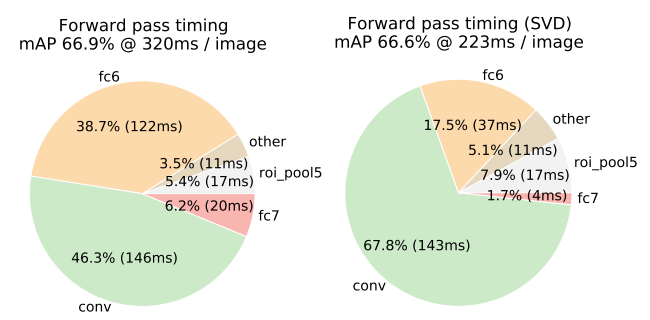
\includegraphics[width=.8\textwidth]{fig2.png}
    \label{fig:img2}
    \caption{Faster R-CNN是一个物体检测的单一统一网络。RPN模块作为这个统一网络的“注意力”。}
\end{figure}

\subsection{候选区域生成网络}

候选区域生成网络(RPN)使用一张图片(任意大小)作为输入并输出一个矩形物体候选的集合,每个候选都有一个置信度。我们使用全卷积网络\cite{fcn}为这个过程建模,这也是我们将在这一章描述的内容。由于我们最终的目标是和Fast R-CNN物体检测网络\cite{fastrcnn}共享计算,因此我们假设两个网络共享一些共同的卷积层。在我们的实验中,我们探讨了有5层共享卷积层的Zeiler和Fergus模型\cite{zf}(ZF)和有13层共享卷积层的Simonyan和Zisserman模型\cite{vgg}(VGG-16)。

为了生成候选区域,我们我们在有最后的共享卷积层输出的卷积特征图上滑动一个小网络。这个小网络使用一个输入卷积特征图的$n\times n$滑动窗口作为输入。每个滑动窗口被映射至一个更低维度的特征(ZF是256维,VGG是512维,并通过ReLU\cite{relu})。这个特征被送入两个孪生全连接层——一个框回归层(\textit{reg})和一个框分类层(\textit{cls})。我们在这片文章中使用$n=3$,注意输入图片的有效接受域是很大的(ZF和VGG分别是171和228像素)。这个迷你网络在图\ref{fig:img3}的左边被单独阐述。注意由于迷你网络通过滑动窗口的方式操作,所以全连接网络被所有空间位置共享。这种架构自然地被通过$n \times n$卷积层紧接两个$1\times 1$卷积层实现(分别为了\textit{reg}和\textit{cls})。

\begin{figure}[bh]
    \centering
    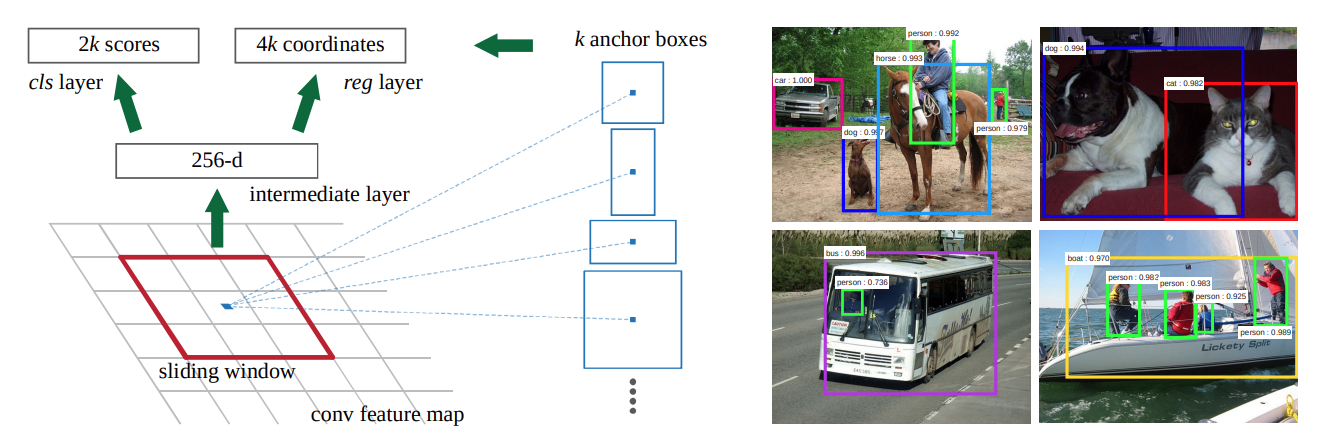
\includegraphics[width=.8\textwidth]{fig3.png}
    \label{fig:img3}
    \caption{\textbf{左}:候选区域生成网络(RPN)。\textbf{右}:在PASCAL VOC 2007 test上使用RPN候选区域的检测例子。我们的方法在大范围的尺度和高宽比上进行了检测。}
\end{figure}

\subsubsection{锚}

在每一个滑动窗口位置,我们同时预测多个候选区域,其中每一个位置的最大可能候选区域数量记为$k$。所以\textit{reg}层有$4k$个输出来编码$k$个框的坐标,\textit{cls}层输出$2k$个值来为每个候选估计是否存在物体的概率。$k$个候选区域相对于$k$个参考框被参数化,我们将之称为\textit{锚}。锚的中心在滑动窗口的某个位置,并与尺寸和高宽比关联(图\ref{fig:img3}左)。我们默认使用3个尺寸和3个高宽比,在每个滑动位置得到$k=9$个锚。对于一个尺寸为$W\times H$(典型大致为2400)的卷积特征图,共有$WHk$个锚。

\paragraph*{具有转变不变形的锚}

我们的方法的一个重要性质就是它的\textit{转变不变性},就锚和计算关于锚的候选的函数来说都是如此。如果对图片中的一个物体进行转变,那么候选也应该转变,同时同样的函数应该可以在一个位置预测候选区域。这个转变不变性性质由我们的方法保证。与之对比的是,MultiBox方法\cite{multiBox1, multiBox2}使用k-means来生成800个锚,这\textit{不是}转变不变性的。所以当一个物体转变时,MultiBox并不能保证生成同样的候选区域。

转变不变性也减少了模型大小。MultiBox有一个$(4 + 1) \times 800$维的全连接输出层,然而我们的方法在$k=9$时仅有一个$(4 + 2) \times 9$维的卷积输出层。作为结果,我们的输出层有$2.8 \times 10^4$个参数(对于VGG-16来说,$512 \times (4 + 2) \times 9$),比有$6.1 \times 10^6$(对于MultiBox中的GoogleNet,$1536\times (4+1)\times 800$)个参数的MultiBox的输出层小两个数量级。如果考虑特征映射层,我们的候选区域生成层参数数量仍然比MultiBox的参数数量小一个数量级。我们期待我们的模型在小数据集上,例如PASCAL VOC,过拟合的风险更小。

\paragraph*{作为回归参考的多尺度锚}

我们对于锚的设计展示了一种创新的解决多尺度(和高宽比)问题的方案。如图\ref{fig:img1}所示,存在两种多尺度预测的方式。第一种方式基于图片/特征金字塔,例如,DPM\cite{dpm}和基于CNN的方法\cite{overfeat, rcnn, fastrcnn}。图片被重塑为多个尺寸,并未每个尺寸计算特征图(HOG\cite{dpm}或者深度卷积特征\cite{overfeat, rcnn, fastrcnn})(图\ref{fig:img1}(a))。这种方式通常是有效的,但是耗费时间。第二种方式是使用多个尺寸(和/或高宽比)的滑动窗口。例如,在DPM\cite{dpm}中,不同高宽比的模型使用不同的过滤器尺寸分别进行训练(例如$5\times 7$和$7\times 5$)。如果使用这种方式来攫夺多尺度问题,它可以被想象为“过滤器金字塔”(图\ref{fig:img1}(b))。第二种方式通常与第一种方式结合使用。

作为比较,我们的基于锚的方式是在\textit{锚金字塔}上构建的,同时也是最花费高效的。我们的方法使用多个尺寸和高宽比的锚作为参考来分类并回归边界框。它仅依赖于单一尺寸的图片和特征图,并使用单一尺寸的过滤器(特征图上的滑动窗口)。我们通过实验展示了这种方案对于解决多尺度和多大小的作用。

由于这个多尺度设计基于锚,所以我们可以简单地使用在单一尺度图片上计算得到的卷积特征,正如Fast R-CNN\cite{fastrcnn}中所做的。多尺度锚的设计是在无额外开销的情况下共享特征来解决尺度问题的关键组成成分。

\subsubsection{损失函数}

为了训练RPN,我们为每一个锚分配了一个二进制类别标签(是否是一个物体)。我们为两种锚分配正标签:(i)与ground-truth框有最大IoU的锚(们)或(ii)与任意ground-truth框的IoU高于0.7的锚。注意一个ground-truth框可能会为多个锚分配正标签。通常第二种情况对于决定正样本来说已经足够了;但是在某些罕见情况下,第二个条件可能会找不到正样本,所以我们任然采用了第一个条件。如果锚与任意ground-truth框的IoU都低于0.3,我们为其分配负标签。既不是正例也不是负例的锚不会对训练目标做出贡献。

有了这些定义,我们最小化一个遵循Fast R-CNN\cite{fastrcnn}中的多任务损失的目标函数。我们对于单张图片的损失函数定义为:
\begin{equation}
    L(\{p_i\}, \{t_i\}) = \frac{1}{N_{cls}}\sum_i L_{cls}(p_i, p_i^*) + \lambda \frac{1}{N_{reg}}\sum_i L_{reg}(t_i, t_i^*)
\end{equation}
这里,$i$是迷你批中的一个锚的索引,$p_i$是预测的锚$i$是一个物体的概率。当锚是正例是ground-truth的标签为1,如果锚是负例则为0。$t_i$表示预测边界框的4个参数化坐标,$t_i^*$则是与一个正例锚相关联的ground-truth框。分类损失$L_{cls}$是两个类别(是否有物体)的对数损失。对于回归损失,我们使用$L_{reg}(t_i, t_i^*)=R(t_i-t_i^*)$,其中$R$是\cite{fastrcnn}中定义的鲁棒损失函数(平滑$L_1$)。$p_i^*L_{reg}$项表示回归损失仅在正例锚($p_I^*=1$)作用,而在其他情况不作用。\textit{cls}和\textit{reg}层的输出分别组成了$\{p_i\}$和$\{t_i\}$。

对于边界框回归,我们遵循\cite{rcnn},采用了如下所示的四个坐标的参数化:
\begin{equation}
    \begin{aligned}
         & t_x = (x - x_a) / w_a,     & t_y = (y - y_a) / h_a,     \\
         & t_w = \log(w/w_a),         & t_h = \log(h/h_a)          \\
         & t_x^* = (x^* - x_a) / w_a, & t_y^* = (y^* - y_a) / h_a, \\
         & t_w^* = \log(w^*/w_a),     & t_h^* = \log(h^*/h_a),
    \end{aligned}
\end{equation}
其中$x, y, w$和$h$表示框的中心坐标以及它的宽度和高度。变量$x, x_a$和$x^*$分别表示预测框,锚框和ground-truth框($y,w,h$类似)。这可以被想象为从锚框到附近ground-truth框的边界框回归。

不仅如此,我们的方法通过不同于以往基于ROI(Region of Interest,感兴趣区域)方法的方式\cite{spp, fastrcnn}来实现边界框回归。在\cite{spp, fastrcnn}中,边界框回归是在从\textit{任意}尺寸ROI池化得到的特征上进行的,同时所有区域尺寸共享回归的权重。在我们的提法中,用于回归的特征在特征图上都有\textit{相同}的空间大小($3\times 3$)。为了考虑变化的尺寸,会习得$k$个边界框回归器。每个回归器为一个尺寸和高宽比负责,同时$k$个回归器\textit{不会}共享权重。这样一来,即使特征是固定尺寸,感谢锚的设计,我们仍然有可能预测不同尺寸的框。

\subsubsection{训练RPN}

我们可以通过反向传播和随机梯度下降(SGD)训练RPN。我们遵循\cite{fastrcnn}中的“以图片为中心”的采样策略来训练网络。每个来自单一图片的迷你批包含多个正例和负例锚。虽然优化考虑所有锚的损失函数是可能的,但是由于负例样本占绝大多数,这会向负例样本偏移。取而代之的是,我们在一张图中随机采样256个锚来计算迷你批的损失函数,其中正例和负例的锚的比例\textit{最多}为$1:1$。如果图片中的正例样本比128少,我们将会使用负例来填充。

我们使用来自均值为0、标准差为0.01的高斯分布的权重来初始化所有的新层。正如标准做法\cite{rcnn},所有其他的层(也就是,共享的卷积层)通过在ImageNet分类任务上训练得到的模型初始化。我们调整ZF网络的所有层和VGG网络conv3\_1及其后续层来节省内存\cite{fastrcnn}。在PASCAL VOC数据集上,我们对前60k个迷你批使用0.001的学习率,接下来20k个迷你批则使用0.0001的学习率。我们使用0.9作为动量以及0.0005的权重衰减\cite{alexnet}。我们使用Caffe实现。

\subsection{RPN和Fast R-CNN的共享特征}

到此为止我们已经描述了如何训练生成候选区域的网络,但是还没有考虑将会使用这些候选区域的基于区域的物体检测CNN。对于检测网络,我们采用Fast R-CNN\cite{fastrcnn}。接下来我们描述学习一个由共享卷积层的RPN和Fast R-CNN组成的统一网络(图\ref{fig:img2})的算法。

独立训练的RPN和Fast R-CNN都会通过不同的方式修改它们的卷积层。因此我们需要开发一种允许在两个网络间共享卷积层而不是学习两个分开网络的技术。我们讨论三种训练共享特征网络的方法:

(i)\textit{依次训练}。在这种方案中,我们先训练RPN,并使用候选区域训练Fast R-CNN。被Fast R-CNN调整的网络接着被用来初始化RPN,接着进行迭代这个过程。这是在论文所有实验中使用的方法。

(ii)\textit{近似联合学习}。在这种方案中,如图\ref{fig:img2}所示,RPN和Fast R-CNN网络将会在训练中合并如一个网络。在每一个SGD迭代中,前向传播会生成在训练Fast R-CNN检测器被视为固定的、事先计算好的候选区域的候选区域。反向传播照常进行,其中共享层的传播信号将来自RPN和Fast R-CNN的损失结合。这种方案实现起来是简单的。但是这种方案忽视了作为网络响应的候选区域坐标的衍生物,所以是近似的。在我们的实验中,我们经验性地发现这种解决方案产生近似的结果,然而与依次训练相比,减少了$25-50\%$的训练时间。我们发布的Python代码中包含了这种解决方案。

(iii)\textit{非近似联合学习}。正如上面讨论的,RPN预测的边界框也是函数的输入。Fast R-CNN中的ROI池化层接受卷积特征以及预测的边界框作为输入,所以一个理论可行的反向传播解决方案应该也考虑到框坐标的梯度。这些梯度在上述的近似联合学习中被忽视。在非近似联合学习中,我们需要一个对框坐标可导的RoI池化层。这并不是一个轻松的问题,可以通过\cite{15}提出的“ROI包裹”层给出一种解决方案,但是这超出了本文的讨论范围。

\textbf{4步依次训练。}在这片论文中,我们采用了使用的4步训练算法来通过依次优化习得共享特征。在第一步中,我们如3.1.3节中所描述的那样训练一个RPN。这个网络使用ImageNet预训练模型初始化并在候选区域生成任务上微调。在第二步中,我们使用第一步得到的RPN生成的候选区域训练一个单独的Fast R-CNN检测器。这个检测网络也通过ImageNet预训练模型初始化。在这个节点,两个网络并没有共享卷积层。在第三步,我们使用检测网络来初始化RPN训练,但是我们固定共享的卷积层并只微调RPN特有的层。现在两个网络共享一些卷积层了。最终,保持共享的卷积层固定,我们微调Fast R-CNN的特有卷积层。这样一来,两个网络共享相同的卷积层并形成了一个统一网络。类似的依次训练可以重复多次,但是我们发现收效甚微。

\subsection{实现细节}



\end{document}